
\chapter{Correcciones atmosféricas}
El objetivo de esta clase es estudiar los efectos de la atmósfera sobre los parametros ópticos y biofísicos obtenidos a partir de una imagen satelital.

\section{Efecto de no conciderar la atmósfera}

Para motivar la necesidad de realizar correcciones atmosféricas a las imágenes es de utilidad observar cual es el efecto de trabajar a tope de la atmósfera para dos situaciones:

\begin{itemize}
    \item La extracción de firmas espectrales.
    \item La estimación de variables biofísicas.
\end{itemize}

\subsection{Comparación de firmas espectrales}

Abra las imágenes \path{S2A_MSIL1C_20161212} y \path{S2A_MSIL2A_20161212} que se encuentran en la carpeta \path{material/raster_data}. La primera corresponde a las reflectancias a tope de la atmósfera mientras que la segunda corresponde a las reflectancias corregidas atmosfericamente.

Desplieguelas y comparelas visualmente. Sobre la imagen corregida hubique \emph{pins} en distintas coberturas. Incluya al menos una cobertura vegetal, una de agua y una de suelo desnudo. Observe las firmas espectrales en dicha imagen para las distintass coberturas. Exporte luego estos valores a un archivo \path{.csv} utilizando la opción \emph{Export spectra to text file}.

Desde el \emph{Pin manager} es posible copiar los \emph{pins} a otra imagen utilizando la herramienta \emph{Transfer the selected pins to other product}. Utilicela y copie los pins a la imagen a tope de la atmósfera.

Obtenga ahora la firma espectral para los \emph{pins} en la imagen no corregida y exportelas a un archivo \emph{.csv}.

Abra ambos en una planilla de calculo y gráfique en conjunto las firmas espectrales a tope de la atmósfera y corregidas (Figura \ref{fig:firmas}). Deberá eliminar la banda de los $1374nm$ cuya única utilidad es realizar correcciones atmosfericas.

\begin{figure}[h!]
    \centering
    %\includegraphics{fig:firmas.png}
    \caption{}
    \label{fig:firmas}
\end{figure}

\begin{que}
    ¿Que diferencia nota entre las dos firmas? ¿En que zona es mayor la diferencia? ¿Que sucede en el infrarrojo medio? ¿Que sucede en la banda de los $945nm$? ¿Que efecto atmosférico domina en casa zona?
\end{que}

\subsection{Estimación de variables biofísicas}

Calcule el SAVI para ambas imágenes y luego utilice el modelo obtenido para el LAI en la clase anterior para estimar el LAI en la nueva fecha. Recuerde utilizar

\begin{equation}
    \beta = \frac{\nu - b}{m}
\end{equation}

con $b = 0.23$ y $m=0.11$. Compare visualmente ambas imágenes. Calcule luego la diferencia entre ambas bandas y gráfique el histograma para dicha diferencia (Figura \ref{fig:hist}).

\begin{figure}[h!]
    \centering
    %\includegraphics{fig:hist.png}
    \caption{}
    \label{fig:hist}
\end{figure}

\begin{que}
    ¿Que regiones de la imagen presentan mayor diferencia? ¿Que regiones menos? ¿Es la diferencia uniforme a lo largo de la imagen? ¿Que diferencia observa en el histograma? ¿Es uniforme? ¿Cual es la difrencia promedio? ¿Coinciden los valores obtenidos utilizando la imagen corregida y no corregida? ¿Cómo es el histograma de la diferencia porcentual?
\end{que}

\section{Corrección por simple dos}

El metodo de corrección por substracción de cuerpo obscuro (simple dos) consiste en restar a cada banda su valor mínimo, estimando que dicho valor coincide con la radiancia de camino debída a la atmósfera. Este método funcionará mejor en los cosas donde haya un cuerpo de reflectancia nula o casi nula.

Para aplicarlo comenzamos obteniendo el valor mínimo de reflectancia utilizando la herramienta \emph{Statistics} para todas las bandas salvo la de los $1374nm$ . Gráficamos dicho valor como función de la longitud de onda (Figura \ref{fig:rlambda}) utilizando el archivo \path{dos.xlsx} de la carpeta \path{material/aux_data}

\begin{figure}[h!]
    \centering
    %\includegraphics{fig:rlambda.png}
    \caption{}
    \label{fig:rlambda}
\end{figure}

Corrija ahora la imagen por el método de simple DOS utilizando la herramienta \emph{Band math...}. La formula a utilizar es

\begin{equation}
    \rho_{sdos} = \rho_{toa} - \rho_{A} + 0.01
\end{equation}

donde $\rho_{A}$ corresponde a la reflectancia ajustada obtenida de la planilla de Excel. Por ejemplo, para corregir la banda uno utilice

\begin{verbatim}
    B1 - 0.09 + 0.01
\end{verbatim}

Configure además en \emph{Band math...} los parametros como

\begin{itemize}
    \item name: sdos\_B1
    \item Unit: dl
    \item Spectral wavelength: 443.0
\end{itemize}

Cambiando la longitud de onda y la banda para cada banda (Figura \emph{fig:sdosbm}).

\begin{figure}[h!]
    \centering
    %\includegraphics{fig:sdosbm.png}
    \caption{}
    \label{fig:sdosbm}
\end{figure}

\begin{que}
    ¿En que zonas del espectro electromagnético es más grande el cambio? ¿Cómo se comporta la reflectancia mínima con la longitud de onda? ¿Que le dice el valor del exponente de decaimiento sobre la atmósfera?
\end{que}

\section{Corrección por 6S}

Para realizar la corrección utilizando el 6S es necesario no solamente contar con la imagen, sino también con datos del satélite y atmosféricos que le permitan simular las condiciones de la atmósfera.

Para los datos del satélite, es necesario conocer los centros y anchos de banda para cada una de las bandas. Estos pueden encontrarse en \href{https://goo.gl/epQ6cw}. De la tabla para cada una de las longitudes de onda puede obtenerse los valores minimos y máximos de la función de respuesta del sensor como

\begin{equation}
    \lambda_{min} = \lambda_{c} - \Delta \lambda /2
\end{equation}

y

\begin{equation}
    \lambda_{min} = \lambda_{c} + \Delta \lambda /2
\end{equation}

con $\lambda_c$ la longitud de onda central \footnote{Central wavelength} y $\Delta \lambda$ el ancho de banda \footnote{Bandwidth}.

Además necesitará la visibilidad que puede obtener para la fecha de la imagen de \href{https://goo.gl/6ozXfH}.

Ingrese a la página de 6S en \href{http://6s.ltdri.org/pages/run6SV.html} y haga click en \emph{Submit} para iniciar el proceso de corrección (Figura \ref{fig:s61}).

\begin{figure}[h!]
    \centering
    %\includegraphics{fig:s61.png}
    \caption{}
    \label{fig:s61}
\end{figure}

Elija luego el paso \emph{1. Geometric conditions} para comenzar a configurar el 6S. Seleccione \emph{User's} y haga click en submit.

Cuando aparezca la página \emph{User's Geometrical Conditions} ponga el més y el día de la imagen. Obtenga luego los parametros de ángulos cenitales y asimutales para el sol y el sensor calculando los promedios de \emph{sun\_zenit}, \emph{sun\_azimuth}, \emph{view\_zenith\_mean} y \emph{view\_azimuth\_mean} (Figura \ref{fig:6sgeo}).  Haga luego click en submit.

\begin{figure}[h!]
    \centering
    %\includegraphics{fig:6sgeo.png}
    \caption{}
    \label{fig:6sgeo}
\end{figure}

Seleccione a continuación \emph{2. Atmospheric model}. Seleccione para el \emph{Atmospheric profile} del menú desplegable \emph{Midlatitude Summer} y del \emph{Aerosol Model}  la opción \emph{Continental model} (Figura \ref{fig:6satmo}).

\begin{figure}[h!]
    \centering
    %\includegraphics{fig:6satmo.png}
    \caption{}
    \label{fig:6satmo}
\end{figure}

Cuando le pregunte \emph{AOT o Visibility} seleccione \emph{Visibility (km)} del menú e ingrese el valor meteorológico obtenido.

Seleccione luego \emph{3. Target Sensor Altitude} elija \emph{Sea level} para el \emph{Target altitude} y \emph{Satellite level} para \emph{Sensor altitude} (Figura \ref{fig:6salt}) haga luego click en submit.

\begin{figure}[h!]
    \centering
    %\includegraphics{fig:6salt.png}
    \caption{}
    \label{fig:6salt}
\end{figure}

Seleccione luego \emph{4. Spectral Conditions}. Elija en \emph{Spectraal conditions} la opción \emph{Same filter function=1} (Figura \ref{fig:6sspec})

\begin{figure}[h!]
    \centering
    %\includegraphics{fig:6sspec.png}
    \caption{}
    \label{fig:6sspec}
\end{figure}

haga click en \emph{submit}, ingrese los valores mínimos y máximos para longitud de onda de la banda 1 \footnote{Recuerde convertirla en $\mu m$.} (Figura \ref{fig:6smm})

\begin{figure}[h!]
    \centering
    %\includegraphics{fig:6smm.png}
    \caption{}
    \label{fig:6smm}
\end{figure}

Configure luego la opción \emph{5. Ground Reflectance} dejando la configuración por defecto y poniendo $0$ cuando le pregunte \emph{input constant value for ro}.

Por ultimo en \emph{6. Signal} deje los valores por defecto. Haga click en submit nuevamente y por último seleccione \emph{7. Results}. Habra el \emph{Output file} (Figura \ref{fig:6sres})

\begin{figure}[h!]
    \centering
    %\includegraphics{fig:6sres.png}
    \caption{}
    \label{fig:6sres}
\end{figure}

Y del archivo de texto obtenido anote los parámetros:

\begin{itemize}
    \item \texttt{global gas. trans. :} de la columna \texttt{total} ($\alpha$)
    \item \texttt{total  sca.   "    :} de la columna \texttt{total} ($\beta$)
    \item \texttt{spherical albedo   :} de la columna \texttt{total} ($\gamma$)
    \item \texttt{reflectance I      :} de la columna \texttt{total} ($\rho_I$)
\end{itemize}

Repita el procecso para todas las bandas salvo la 10.

Una vez obtenidos los parametros de arriba para cada banda, puede corregir la imagen utilizando la ecuación

\begin{equation}
    \rho_{sdos} = \frac{\frac{\rho_{toa}}{\alpha \beta} - \frac{\rho_I}{\beta}}{1+\gamma \left(\frac{\rho_{toa}}{\alpha \beta} - \frac{\rho_I}{\beta}\right)}
\end{equation}

\begin{que}
    ¿Que zonas del espectro presentan más cambio? ¿Donde aumenta la reflectancia y donde disminuye? ¿A que fenomeno de interacción entre la luz y la atmósfera se debe cada cambio?
\end{que}

\section{Comparación entre los resultados TOA y corregidos}

Hasta este momento traabajo con bandas virtuales dentro de \emph{SNAP}. Al utilizarlas no se calculan hasta que no hace falta mostrar la información. Puede forzar a que el software las calcule haciendo click derecho sobre la banda y eligiendo la opción \emph{Convert band}. Convierta todas las bandas que generó en las clases anteriores.

Utilice la herramienta \emph{Raster/Subset} y en \emph{Band subset} seleccione solo las bandas correspondientes a la corrección por simple dos (Figura \ref{fig:subset}). Repita el proceso utilizando solo las bandas obtenidas utilizando el 6S web.

\begin{figure}[h!]
    \centering
    %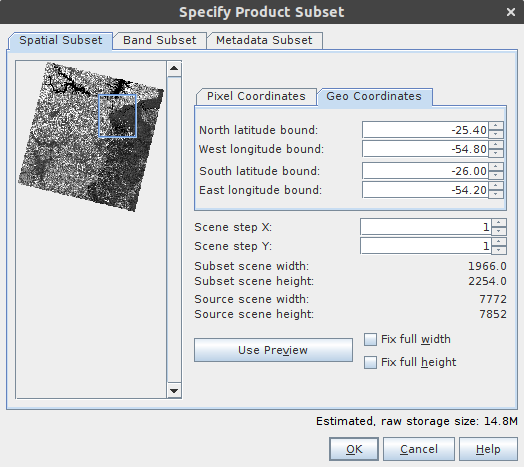
\includegraphics{fig:subset.png}
    \caption{}
    \label{fig:subset}
\end{figure}

Con las dos nuevas imágenes obtenidas, calcule las firmas espectrales y utilizando el modelo obtenido para el SAVI, el LAI que obtendría de cada una.

Compare los resultados con los obtenidos en la sección 1.

\begin{que}
    ¿Como se comparan las firmas espectrales de las imagenes corregidas con la imagen TOA?¿Cual es la diferencia promedio entre el SAVI para cada tipo de corrección?
\end{que}
